%!TEX root = ../thesis.tex

\section{関連研究}\label{sec:relate-research}
近年,歩行者の複雑な動きを予測するために,深層学習を応用しようとする研究が注目を集めている.
深層学習を歩行者の軌道予測に応用した例として,Alexandreら\cite{s-lstm}は,人間の動きを学習し,将来の軌跡を予測できるLSTMモデルを提案した.Social-LSTMは,歩行者の軌道予測に着目した最も初期の深層学習モデルの一つである.Social-LSTMは,\figref{Fig:s-lstm}のように各歩行者の軌跡ごとに1つのLSTMを割り当て,プーリング機構を通じて複数のLSTM間で情報を共有することで,歩行者間の相互作用を捉えることを可能にしている.このシステムにより,複数の個人にわたって相互作用から生じるさまざまな非線形行動をうまく予測することに成功した.

\vspace{-10pt}

\begin{figure}[hbtp]
     \centering
    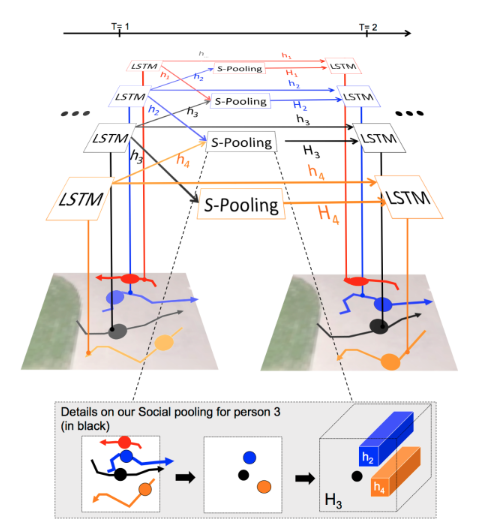
\includegraphics[keepaspectratio, scale=0.55]
         {images/s-lstm.png}
    \caption{Overview of Social-LSTM method.\protect\footnotemark[1]}
    \label{Fig:s-lstm}
\end{figure}
\protect\footnotetext[1]{\cite{s-lstm}より引用}

% \newpage

Zhangら\cite{sr-lstm}は,LSTMのシーケンス学習能力にエージェント間の相互作用をモデル化するため,\figref{Fig:sr-lstm-str}のようなLSTMネットワークの情報精密化モジュールを提案している.この研究では,Attention機構により,各歩行者の他者への影響を重み付けしている.この手法により,\figref{Fig:sr-lstm}のように近隣の歩行者に対してより注意を向けるよう学習することが可能になる.

% \vspace{0.8zh}

\begin{figure}[hbtp]
     \centering
    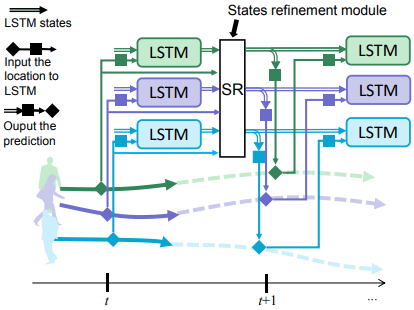
\includegraphics[keepaspectratio, scale=0.6]
         {images/sr-lstm-str.png}
    \caption{Framework overview of proposed SR-LSTM.\protect\footnotemark[2]}
    \label{Fig:sr-lstm-str}
\end{figure}

% \vspace{-10pt}

\begin{figure}[hbtp]
     \centering
    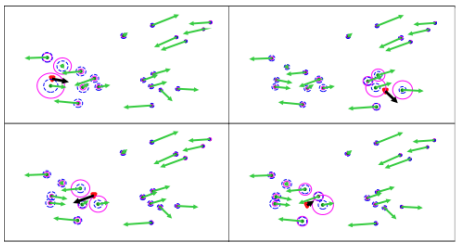
\includegraphics[keepaspectratio, scale=0.6]
         {images/sr-lstm.png}
    \caption{Illustration of the pedestrian-wise attention.\protect\footnotemark[2]}
    \label{Fig:sr-lstm}
\end{figure}

\protect\footnotetext[2]{\cite{sr-lstm}より引用}

同様に,歩行者の注意に着目した研究をKosarajuら\cite{s-bigat}も行っている.この研究は,LSTMを用いて各歩行者の軌跡をモデル化し,グラフアテンションネットワーク(GAT)を用いて,現実的な歩行者の軌道予測を実現している.この研究では,グラフは\figref{Fig:s-bigat}のように歩行者をノード,距離をエッジとしてモデル化される.このグラフ構造を用いることで,歩行者間の相互作用を効果的に捉え,より正確な軌道予測が可能となる.
\vspace{20pt}
\begin{figure}[hbtp]
     \centering
    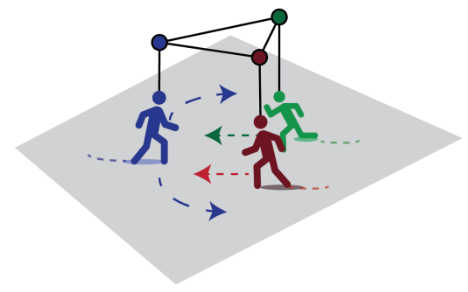
\includegraphics[keepaspectratio, scale=0.4]
         {images/s-bigat.png}
\caption{Illustration of the pedestrian-wise dependencies.\protect\footnotemark[3]}
    \label{Fig:s-bigat}
\end{figure}

\protect\footnotetext[3]{\cite{s-bigat}より引用}

また,Mohanmedら\cite{s-stgcnn}は軌跡をグラフとしてモデル化し,歩行者間のユークリッド距離で重み付けされたエッジは歩行者間の相互作用を表している.\figref{Fig:s-stgcnn}のように,モデルはグラフ畳み込みニューラルネットワークと時間畳み込みネットワーク(TCN)を用いて,時空間グラフ上で動作し,一度にシーケンス全体を予測できるようにしている.

\vspace{20pt}

\begin{figure}[hbtp]
     \centering
    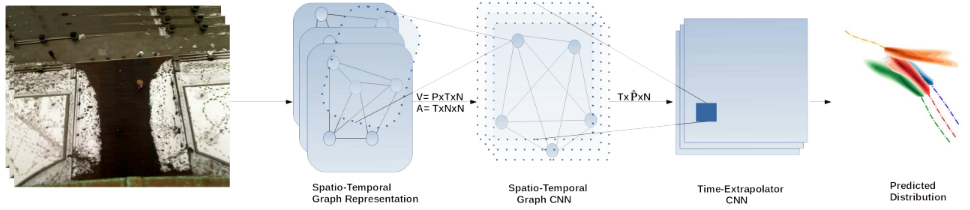
\includegraphics[keepaspectratio, scale=0.39]
         {images/s-stgcnn.png}
    \caption{The Social-STGCNN model.\protect\footnotemark[4]}
    \label{Fig:s-stgcnn}
\end{figure}

\protect\footnotetext[4]{\cite{s-stgcnn}より引用}

\newpage

移動ロボットで歩行者の軌道予測を行う場合,歩行者同士の相互作用の他にロボットと人間にも相互作用が存在する.そのため,歩行者だけでなくロボットの行動も考慮した軌道予測手法が求められる.

丹野ら\cite{si2023-tanno}は,歩行者の軌道予測に過去の動きだけでなく,\figref{Fig:future-robot}に示すようにロボットが選択する将来の動きを考慮して予測をする手法を提案している.実験では,ロボットの将来の行動を考慮しない場合と比較して,ロボットの動きに応じて変化する歩行者の動きを予測できることが確認されている.しかし,この手法では学習器の事前学習時に,データセット内の歩行者をロボットに置き換えて学習している.すなわち,歩行者の行動がロボットの行動と近似できるという前提のもとでモデルを構築していることになる.この前提に基づけば,モデル構造におけるロボットのエンコード部分を省略し,人間とロボットでネットワークを共有化できる可能性が考えられる.これは,ネットワークの肥大化を防ぐ上で有効である.
本研究では,\ref{chap:experiments_oculus}章においてこの論文\cite{si2023-tanno}を参考に実験を行う.
\begin{figure}[hbtp]
     \centering
    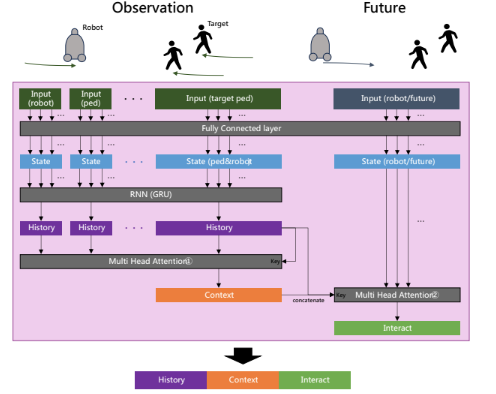
\includegraphics[keepaspectratio, scale=0.64]
         {images/future-robot.png}
    \caption{Encoder structure.\protect\footnotemark[5]}
    \label{Fig:future-robot}
\end{figure}
\protect\footnotetext[5]{\cite{si2023-tanno}より引用}

% このように,深層学習を歩行者の軌道予測タスクに応用する例は少なくない.しかし,その多くは俯瞰図形式のデータセットを用いて学習器を訓練しており,実際の移動ロボットを対象とした研究は少ない.
このように,深層学習を歩行者の軌道予測タスクに応用する例は少なくない.しかし,その多くは俯瞰図形式のデータセットを用いて学習器を訓練しており,実際の屋内外環境で動作する移動ロボットを用いた実験を対象とした研究は少ない.
また,移動ロボットを扱っている場合でも,予測対象の歩行者にトラッキングセンサを取り付けるなど環境に介入している例や,シミュレータから真値を取得しているなど,移動ロボットが収集するセンサデータのみで完結する手法はあまり報告されていない.そのため,深層学習を用いて予測した歩行者の軌道を移動ロボットのナビゲーションに直接活用している研究は,現時点では非常に限られている.

\newpage